\begin{tikzpicture}[
    >=Stealth,
    font=\sffamily\small,
    box/.style={draw=black!70, rounded corners=3pt, thick, fill=white, align=center},
    iconbox/.style={draw=none, fill=none, align=center, inner sep=1pt},
    videobox/.style={draw=blue!60!black, rounded corners=3pt, thick, fill=black!2, align=center, inner sep=2.5pt},
    framebox/.style={draw=teal!60!black, rounded corners=3pt, thick, fill=white, align=center, inner sep=2.5pt},
    stepbox/.style={box, fill=green!12, draw=green!60!black, thick, font=\sffamily\scriptsize, align=center},
    detector/.style={box, fill=cyan!10, draw=cyan!70, font=\sffamily\footnotesize, text width=2.5cm, minimum height=1.05cm},
    fusion/.style={box, fill=purple!10, draw=purple!70, thick, font=\sffamily\footnotesize, text width=2.5cm, minimum height=1.1cm},
    method/.style={box, fill=orange!10, draw=orange!75, thick, font=\sffamily\scriptsize, text width=3.4cm, minimum height=0.72cm},
    decision/.style={box, fill=teal!12, draw=teal!70, thick, font=\sffamily\footnotesize, text width=2.2cm, minimum height=1.05cm},
    eval/.style={box, fill=green!10, draw=green!60!black, thick, font=\sffamily\scriptsize, text width=3.4cm, minimum height=1.25cm},
    kpi/.style={draw=red!70!black, fill=red!5, rounded corners=4pt, thick, align=center, inner sep=3pt, text width=3.2cm},
    stagebox/.style={draw=#1!70!black, fill=#1!3, rounded corners=5pt, thick, inner sep=7pt},
    arrow/.style={->, thick, draw=black!75},
    bluearrow/.style={->, thick, draw=blue!70!black},
    orangearrow/.style={->, thick, draw=orange!80!black},
    greenarrow/.style={->, thick, draw=green!60!black},
    purplearrow/.style={->, thick, draw=purple!80!black},
    sig/.style={font=\fontsize{6pt}{7pt}\selectfont\bfseries, text=black!85},
    ttl/.style={font=\fontsize{6pt}{7pt}\selectfont\bfseries}
]

% =========================================================================
% STAGE 1: GENERATION & DATASET PREPARATION
% =========================================================================

% 1. RGB video prompt (Text File Icon - Scaled down 40%)
\node[iconbox] (prompt_rgb) at (0.8, 5.4) {
    
\includegraphics[height=0.72cm]{figures/icon_lorem_ipsum.png}
};
\node[above=3pt of prompt_rgb, ttl, text=blue!80!black] (lbl_p1) {RGB Video Prompt};
\node[below=2pt of prompt_rgb, font=\fontsize{5pt}{6pt}\selectfont, text=black!65] (sub_p1) {Text Prompt};

% 2. Video Generator LLM (Gemini Icon - Scaled down 40%)
\node[iconbox] (gemini_rgb) at (2.8, 5.4) {
    
\includegraphics[height=0.72cm]{figures/gemini_logo.png}
};
\node[above=3pt of gemini_rgb, ttl, text=purple!80!black] (lbl_g1) {Video Generator LLM};
\node[below=2pt of gemini_rgb, font=\fontsize{5pt}{6pt}\selectfont, text=black!65] (sub_g1) {Gemini 3.8 Flash};

\draw[bluearrow] (prompt_rgb) -- (gemini_rgb);

% 3. 16:9 RGB Videos (Desert & Forest with Striped Bottom)
\node[videobox] (rgb_videos) at (5.2, 5.4) {
    \begin{tabular}{@{}c@{\hspace{3pt}}c@{}}
    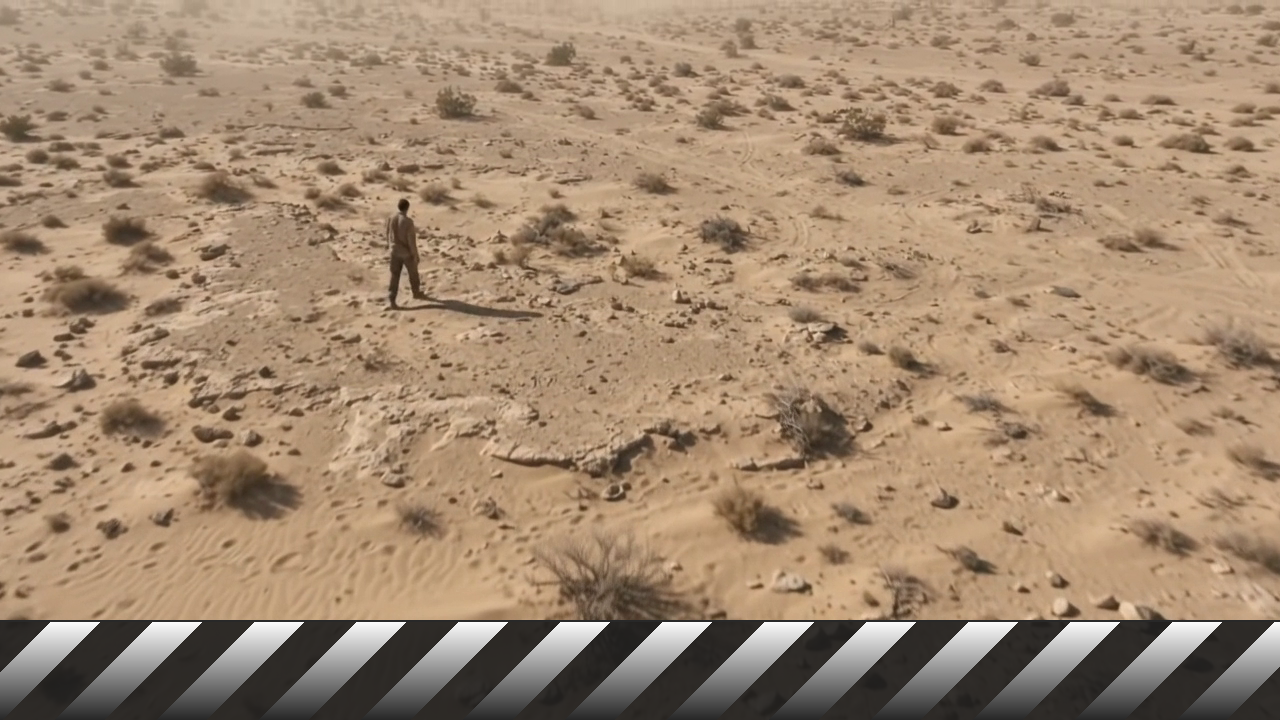
\includegraphics[width=1.15cm]{figures/desert_rgb_video.png} &
    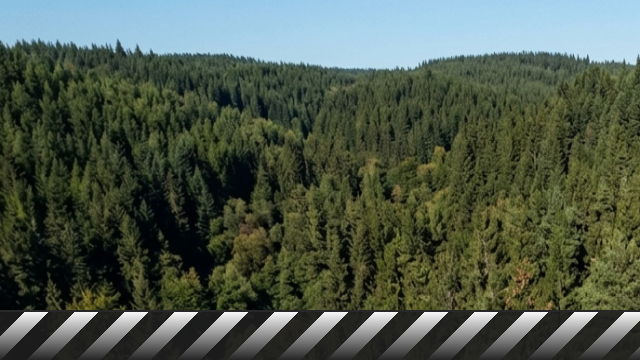
\includegraphics[width=1.15cm]{figures/forest_rgb_video.png} \\
    {\tiny Desert RGB} & {\tiny Forest RGB}
    \end{tabular}
};
\node[above=3pt of rgb_videos, ttl, text=black!85] (lbl_v1) {16:9 RGB Videos};
\node[below=2pt of rgb_videos, font=\fontsize{5pt}{6pt}\selectfont, text=black!60] (sub_v1) {1280$\times$720 @ 24 FPS};

\draw[bluearrow] (gemini_rgb) -- (rgb_videos);

% 4. Configure to Thermal (Text File Icon - Scaled down 40%)
\node[iconbox] (prompt_th) at (7.6, 5.4) {
    
\includegraphics[height=0.72cm]{figures/icon_lorem_ipsum.png}
};
\node[above=3pt of prompt_th, ttl, text=orange!80!black] (lbl_p2) {Configure to Thermal};
\node[below=2pt of prompt_th, font=\fontsize{5pt}{6pt}\selectfont, text=black!65] (sub_p2) {Thermal Prompt};

\draw[orangearrow] (rgb_videos) -- (prompt_th);

% 5. Video Generator LLM (Gemini Icon - Modality Transfer)
\node[iconbox] (gemini_th) at (9.8, 5.4) {
    
\includegraphics[height=0.72cm]{figures/gemini_logo.png}
};
\node[above=3pt of gemini_th, ttl, text=purple!80!black] (lbl_g2) {Video Generator LLM};
\node[below=2pt of gemini_th, font=\fontsize{5pt}{6pt}\selectfont, text=black!65] (sub_g2) {Modality Transfer};

\draw[orangearrow] (prompt_th) -- (gemini_th);

% 6. 16:9 Thermal Videos (Desert & Forest with Striped Bottom)
\node[videobox] (th_videos) at (12.2, 5.4) {
    \begin{tabular}{@{}c@{\hspace{3pt}}c@{}}
    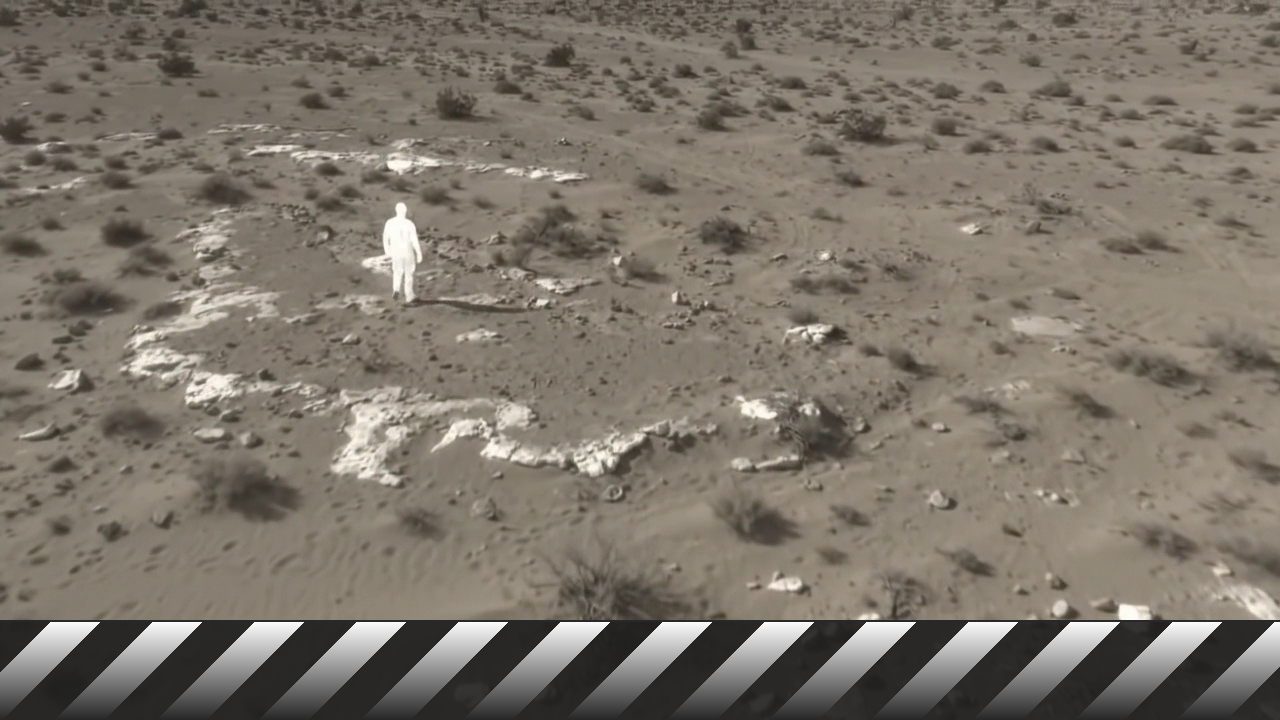
\includegraphics[width=1.15cm]{figures/desert_th_video.png} &
    
\includegraphics[width=1.15cm]{figures/forest_th_video.png} \\
    {\tiny Desert TIR (D:)} & {\tiny Forest TIR}
    \end{tabular}
};
\node[above=3pt of th_videos, ttl, text=black!85] (lbl_v2) {16:9 Thermal Videos};
\node[below=2pt of th_videos, font=\fontsize{5pt}{6pt}\selectfont, text=black!60] (sub_v2) {1280$\times$720 @ 24 FPS};

\draw[orangearrow] (gemini_th) -- (th_videos);

% 7. Crop 640x640 (2 of them: Left & Right Video Snippets)
\node[videobox] (crops) at (14.8, 5.4) {
    \begin{tabular}{@{}c@{\hspace{3pt}}c@{}}
    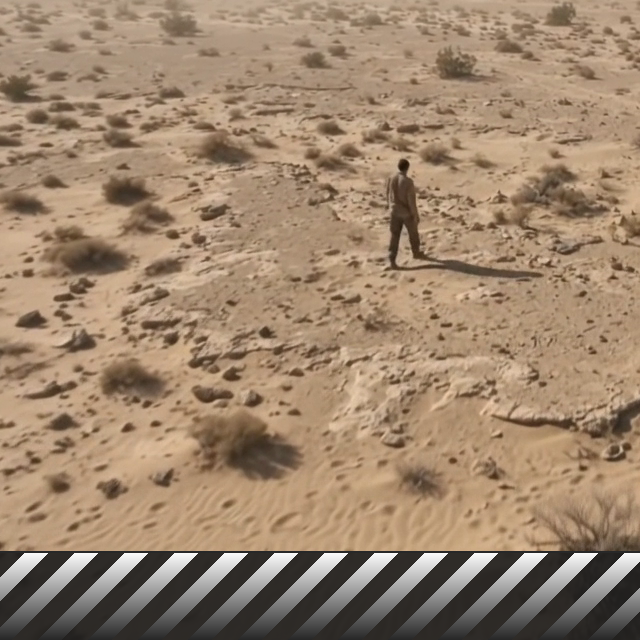
\includegraphics[width=0.82cm]{figures/crop_640_left_video.png} &
    
\includegraphics[width=0.82cm]{figures/crop_640_right_video.png} \\
    {\tiny Left ($x=0$)} & {\tiny Right ($x=640$)}
    \end{tabular}
};
\node[above=3pt of crops, ttl, text=purple!80!black] (lbl_c) {Crop 640$\times$640 (2 Videos)};
\node[below=2pt of crops, font=\fontsize{5pt}{6pt}\selectfont, text=purple!90!black] (sub_c) {Cropped Videos (24 FPS)};

\draw[purplearrow] (th_videos) -- (crops);

% 8. Label Studio Video Annotation (User's uploaded logo - Scaled down 40%)
\node[iconbox] (label_studio) at (17.1, 5.4) {
    
\includegraphics[height=0.72cm]{figures/icon_label_studio.png}
};
\node[above=3pt of label_studio, ttl, text=red!80!black] (lbl_ls) {Label Studio};
\node[below=2pt of label_studio, font=\fontsize{5pt}{6pt}\selectfont, text=black!65] (sub_ls) {Video Annotation};

\draw[purplearrow] (crops) -- (label_studio);

% 9. Video to Frame Decimation & YOLO Export
\node[stepbox, text width=1.35cm] (v2f) at (19.2, 5.4) {
    \textbf{Video to Frame}\\[1pt]
    {\tiny 3:1 Decimation}\\[-1pt]
    {\tiny (24 to 8 Hz)}
};
\node[below=2pt of v2f, font=\fontsize{5pt}{6pt}\selectfont, text=green!60!black] (sub_v2f) {Frame Extraction};

\draw[greenarrow] (label_studio) -- (v2f);

% 10. Annotated Frames (Extracted Clean Frames with YOLO Bounding Boxes)
\node[framebox] (annotated_frames) at (21.4, 5.4) {
    \begin{tabular}{@{}c@{\hspace{3pt}}c@{}}
    
\includegraphics[width=0.88cm]{figures/desert_rgb_annotated.png} &
    
\includegraphics[width=0.88cm]{figures/desert_th_annotated.png} \\
    {\tiny RGB Frame} & {\tiny Thermal Frame}
    \end{tabular}
};
\node[above=3pt of annotated_frames, ttl, text=teal!80!black] (lbl_af) {Annotated Frames};
\node[below=2pt of annotated_frames, font=\fontsize{5pt}{6pt}\selectfont\bfseries, text=teal!90!black] (sub_af) {Dataset Frames};

\draw[greenarrow] (v2f) -- (annotated_frames);

% Stage 1 Background Enclosure & Header Tab
\begin{scope}[on background layer]
    \node[stagebox=blue, fit=(lbl_p1) (sub_p1) (lbl_af) (sub_af) (prompt_rgb) (annotated_frames) (lbl_g1) (lbl_v1) (lbl_p2) (lbl_g2) (lbl_v2) (lbl_c) (lbl_ls) (v2f), inner ysep=8pt, inner xsep=7pt] (stage1) {};
    \node[draw=blue!70!black, fill=blue!15, rounded corners=2pt, font=\sffamily\bfseries\scriptsize, text=blue!90!black, anchor=south west] at ([xshift=4pt, yshift=1pt]stage1.north west) {STAGE 1: GENERATION (SYNTHETIC VIDEO GENERATION, 640$\times$640 DUAL CROPS, LABEL STUDIO \& EXTRACTION)};
\end{scope}

% =========================================================================
% TRANSITION: DATASET REPOSITORY BUS
% =========================================================================

% Dataset Banner in transition gap
\node[draw=purple!70, fill=purple!8, rounded corners=4pt, thick, font=\fontsize{6.5pt}{7.5pt}\selectfont\bfseries, text=purple!90!black] (dataset_banner) at (11.0, 3.6) {
    Harvested MMSAR Benchmark Corpus: 30 Snippets per Environment (60\% Train / 20\% Val / 20\% Test) --- 80 Frames/Clip at 8 Hz
};

% Routing from Stage 1 output to Dataset Banner (clean loop via right margin)
\draw[thick, draw=purple!80, ->] (annotated_frames.east) -- ++(0.35, 0) |- (dataset_banner.east);

% =========================================================================
% STAGE 2: ONBOARD MULTIMODAL DETECTION, DECISION FUSION & CAUSAL POST-PROCESSING
% =========================================================================

% 1. Parallel Detectors (YOLO11n-RGB & YOLO11n-Thermal)
\node[detector] (yolo_rgb) at (2.6, 1.25) {\textbf{RGB Detector}\\[1pt]YOLO11n Backbone\\{\scriptsize 2.6M params, FP32}};
\node[detector] (yolo_tir) at (2.6, -1.25) {\textbf{Thermal Detector}\\[1pt]YOLO11n Backbone\\{\scriptsize 2.6M params, FP32}};

% Internal routing coordinates from Dataset Banner into Stage 2 Detectors
\coordinate (split_bus) at (0.3, 3.6);
\coordinate (in_rgb) at (0.3, 1.25);
\coordinate (in_tir) at (0.3, -1.25);

\draw[thick, draw=purple!80] (dataset_banner.west) -- node[pos=0.5, above=1pt, font=\fontsize{6pt}{7pt}\selectfont\bfseries, text=purple!90!black] {Curated Dataset Stream} (split_bus);
\draw[thick, draw=purple!80] (split_bus) -- (in_rgb);
\draw[thick, draw=purple!80] (in_rgb) -- (in_tir);

\draw[arrow, blue!70!black] (in_rgb) -- node[above=1pt, sig] {RGB 640$\times$640} (yolo_rgb.west);
\draw[arrow, orange!70!black] (in_tir) -- node[below=1pt, sig] {Thermal 640$\times$640} (yolo_tir.west);

% 2. Late Decision Fusion Gate (No equations)
\node[fusion] (fusion) at (6.5, 0) {
    \textbf{Late Decision Fusion}\\[2pt]
    Confidence Max Gate\\[2pt]
    {\scriptsize Soft Disjunctive OR}
};

\draw[arrow, blue!70!black] (yolo_rgb.east) -- node[pos=0.48, above=2pt, sig] {RGB Score} (fusion.north west);
\draw[arrow, orange!70!black] (yolo_tir.east) -- node[pos=0.48, below=2pt, sig] {Thermal Score} (fusion.south west);

% 3. Causal Post-Processing Methods (No equations)
\node[method] (m1) at (11.5, 2.0) {\textbf{M1: Raw Baseline}\\[1pt]Direct Score Threshold\\{\tiny (Instantaneous Confidence)}};
\node[method] (m2) at (11.5, 1.0) {\textbf{M2: Moving Average}\\[1pt]Sliding Window Mean\\{\tiny (5-Frame Window, 625 ms)}};
\node[method] (m3) at (11.5, 0.0) {\textbf{M3: Median Filter}\\[1pt]Order-Statistic Median\\{\tiny (Spike Rejection, 5 Frames)}};
\node[method] (m4) at (11.5, -1.0) {\textbf{M4: History Consensus}\\[1pt]Majority Rule Persistence\\{\tiny (At Least 3 of 5 Detections)}};
\node[method] (m5) at (11.5, -2.0) {\textbf{M5: Learned Mamba-SSSM}\\[1pt]Selective State-Space Filter\\{\tiny (Learned Recurrent Dynamics)}};

% Distribution Bus
\draw[thick, draw=purple!80] (fusion.east) -- (9.2, 0) node[midway, above=2pt, sig, text=purple!90!black] {Fused Score};
\draw[thick, draw=purple!80] (9.2, 2.0) -- (9.2, -2.0);
\draw[arrow, draw=purple!80] (9.2, 2.0) -- (m1.west);
\draw[arrow, draw=purple!80] (9.2, 1.0) -- (m2.west);
\draw[arrow, draw=purple!80] (9.2, 0.0) -- (m3.west);
\draw[arrow, draw=purple!80] (9.2, -1.0) -- (m4.west);
\draw[arrow, draw=purple!80] (9.2, -2.0) -- (m5.west);

% Collection Bus
\draw[thick, draw=teal!80] (13.8, 2.0) -- (13.8, -2.0);
\draw[arrow, draw=teal!80] (m1.east) -- (13.8, 2.0);
\draw[arrow, draw=teal!80] (m2.east) -- (13.8, 1.0);
\draw[arrow, draw=teal!80] (m3.east) -- (13.8, 0.0);
\draw[arrow, draw=teal!80] (m4.east) -- (13.8, -1.0);
\draw[arrow, draw=teal!80] (m5.east) -- (13.8, -2.0);

% 4. Common Alarm Output (No equations)
\node[decision] (alarm) at (15.8, 0) {
    \textbf{Binary Alarm}\\[2pt]
    Verification Gate\\[2pt]
    {\scriptsize Optimal Decision Threshold}
};
\draw[arrow, draw=teal!80, very thick] (13.8, 0) -- (alarm.west);

% 5. Top KPI Formula Callout (Positioned cleanly with 1.1cm clearance above eval)
\node[kpi] (kpi_box) at (20.0, 1.25) {
    \textbf{False Alarm Suppression}\\[1pt]
    {\scriptsize Reduction vs. Raw Baseline}
};
\draw[arrow, draw=red!70!black, thick] (alarm.east) to[out=20, in=180] node[pos=0.55, above=1pt, sig, text=red!80!black] {Alarm Stream} (kpi_box.west);

% 6. Operational Evaluation Framework (Tightened, compact, positioned cleanly below)
\node[eval] (eval) at (20.0, -0.75) {
    \textbf{Operational Evaluation}\\[2pt]
    $\bullet$ Detection Recall, Precision, F1\\
    $\bullet$ False Alarm Suppression\\
    $\bullet$ IoT Telemetry Uplink Savings\\
    $\bullet$ Drone Loiter Energy Savings
};
\draw[arrow, draw=teal!80, very thick] (alarm.east) to[out=-20, in=180] node[pos=0.55, below=1pt, sig, text=teal!90!black] {Alarm Signal} (eval.west);

% Coordinate anchor for stage2 western padding
\coordinate (stage2_w) at (-0.1, 0);

% Stage 2 Background Enclosure & Header Tab
\begin{scope}[on background layer]
    \node[stagebox=green, fit=(stage2_w) (yolo_rgb) (yolo_tir) (eval) (kpi_box) (m1), inner ysep=8pt, inner xsep=7pt] (stage2) {};
    \node[draw=green!60!black, fill=green!15, rounded corners=2pt, font=\sffamily\bfseries\scriptsize, text=green!50!black, anchor=south west] at ([xshift=1.6cm, yshift=1pt]stage2.north west) {STAGE 2: ONBOARD MULTIMODAL DETECTION, DECISION FUSION \& CAUSAL TEMPORAL POST-PROCESSING};
\end{scope}

\end{tikzpicture}
